\section{Methods} \label{sec:methods}

In this Section, we begin with a high-level overview of each variant of the Automap approach.
Then, we discuss two problem domains used to demonstrate these methods --- the $n$-legged table problem and the Scrabble string problem.
We cover the specific implementation of Automap employed in each of those domains.
Finally, we review a visualization technique called the evolvability signature, which we will later use to examine the evolvability properties of genotype-phenotype maps in both problem domains  \cite{tarapore2015evolvability}.

\subsection{Learning an Evolvable Genotype-Phenotype Mapping}

The pair of proposed techniques to automatically learn evolvable genotype-phenotype mappings are based on autoencoders trained to encode phenotypes taken from local fitness peaks spread throughout an evolutionary search space.
(These phenotypes are gathered by evolving a large number of replicate direct-encoded populations and retaining champion individuals from each population).

\begin{figure}
        \begin{subfigure}[b]{0.40\linewidth}
          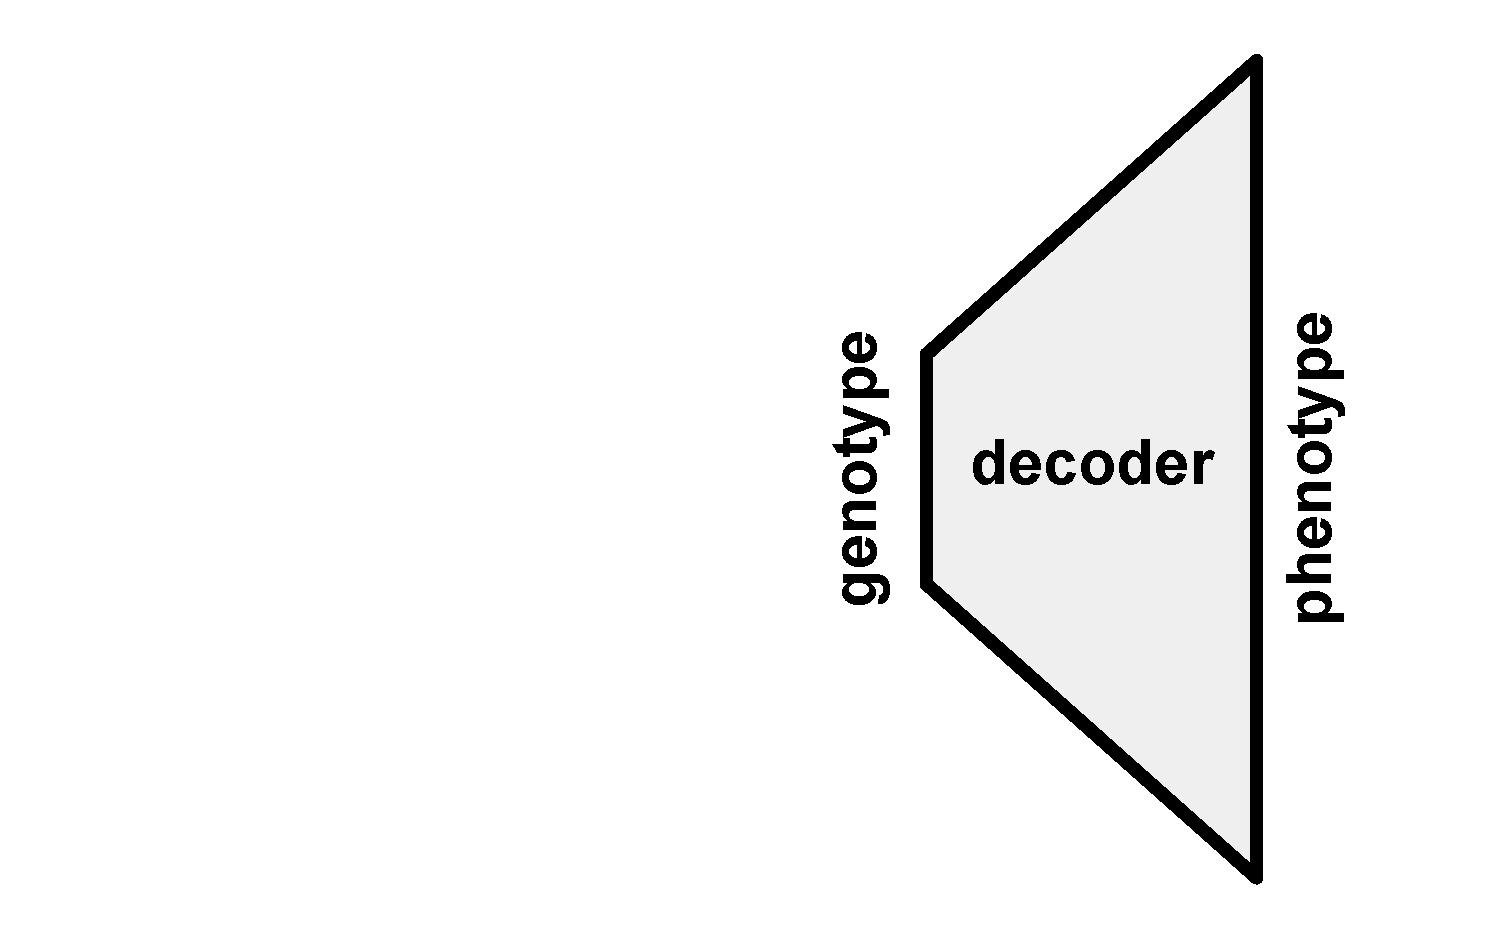
\includegraphics[width=\linewidth]{img/bottleneck_map}
          \subcaption{bottleneck map}
          \label{fig:bottleneck_map}
        \end{subfigure}%
        \begin{subfigure}[b]{0.40\linewidth}
          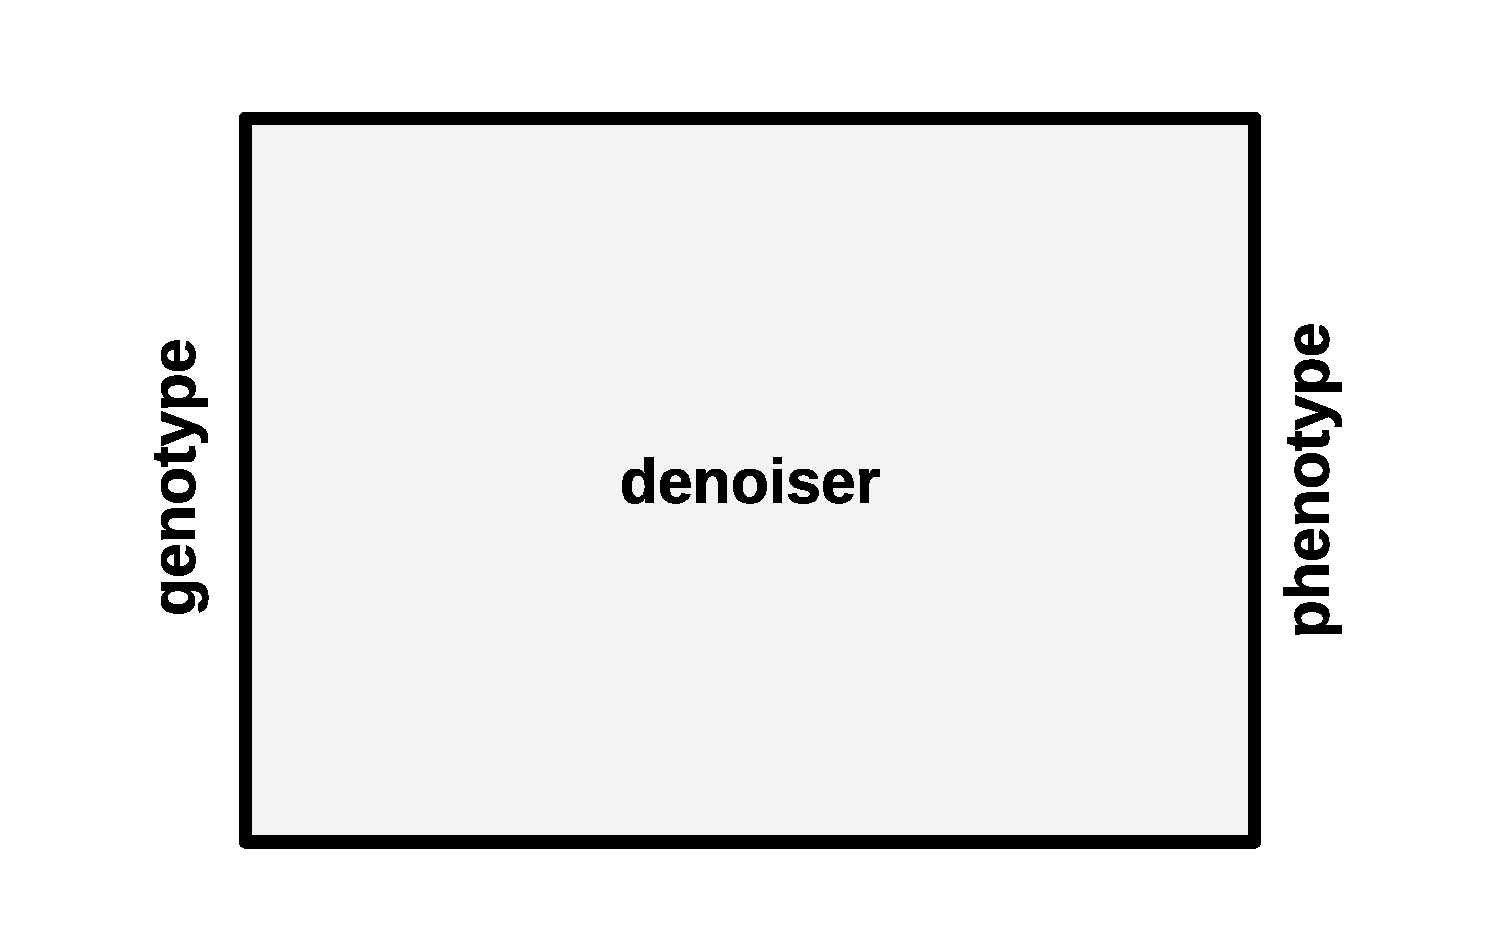
\includegraphics[width=\linewidth]{img/denoiser_map}
          \subcaption{denoiser map}
          \label{fig:denoiser_map}
        \end{subfigure}%
        \caption{Schematics of genotype-phenotype maps constructed with a bottlenecked autoencoder and a denoising autoencoder.}
\label{fig:maps}
\end{figure}


The first approach, the bottleneck map, uses just the decoder portion of the bottleneck autoencoder.
The decoder serves as the genotype-phenotype map so the genotype is now in the bottleneck vector space while the phenotype remains in the same vector space as before.
The idea of this approach is that, because the bottleneck provides a compact representation of those high-fitness phenotypes, using the decoder as a genotype-phenotype mapping will readily allow mutation to move the phenotype between otherwise distant fitness peaks.
Figure \ref{fig:bottleneck_map} illustrates how the decoder component of the bottleneck encoding is employed to define a genotype-phenotype mapping.

The second approach, the denoiser map, employs the entire denoising autoencoder would be used as the genotype-phenotype mapping.
Note that the genotype and phenotype remain in the same, equivalent vector spaces.
The idea of this design is that mutations that would otherwise be deleterious will be interpreted as noise and prevented from being expressed by the genotype-phenotype mapping.
Effectively, this mapping should flatten out the valleys between local fitness peaks to allow evolution to more readily drift between those local fitness peaks.
Figure \ref{fig:denoiser_map} illustrates how the denoiser autoencoder is used to define a genotype-phenotype mapping.

\subsection{$n$-legged Table Problem}

This simple problem is used to present a proof-of-concept for the proposed AutoMap techniques.
The $n$-legged table problem models a table design scenario.
In this problem, the phenotype of a table is nothing more than a collection of continuous-valued individual leg lengths.
All other details of table design are neglected.
Stability is considered a highly-advantageous trait for a table.
The stability of a table is assumed to result solely from uniformity of table leg lengths.
Clearly, as $n$ grows beyond eight or so this toy problem begins to lose a meaningful connection to real world tables.
(When was the last time you saw a fifty-legged table?)
However, mathematically (and intuitively) the $n$-legged table problem scales easily.
We arbitrarily use $n=100$ for all experiments in this domain.

This toy problem was chosen because it creates an easy-to-understand rugged fitness landscape.
Because unstable tables are disadvantageous, mutations to level tables tend to be deleterious.
Thus, evolving between different table heights --- i.e. escaping local maxima --- is a tricky challenge.

For evolvability signature experiments, ``level-ness'' was the sole criterion for fitness.
For a phenotype $\vec{x}$, the fitness score was computed as
\begin{align*}
-\sigma(\vec{x})
\end{align*}
where $\sigma$ represents calculation of standard deviation.
Note that in all experiments performed, selection was performed to maximize (not minimize) fitness score.
Under this criterion, each level table of a particular height is a local fitness peak because any single-site mutation increases the leg height variance.
This fitness criteria was chosen for evolvability signature experiments because of its ruggedness.

For response to selection experiments, the ``level-ness'' and absolute height of a table were both factored into the fitness score.
For a phenotype $\vec{x}$, the fitness score was computed as
\begin{align*}
-\sigma(\vec{x}) - |\mu(\vec{x})/10|
\end{align*}
where $\sigma$ represents calculation of standard deviation and $\mu$ represents calculation of mean.
Under this criterion, a selection pressure for short tables is applied.
The global fitness score peak is the table with all legs length 0.
However, the phenotypic fitness landscape remains rugged with local peaks occurring as before at level tables.
Thus, the ability of genotype-phenotype map to facilitate evolution will be reflected by the ability of a population to escape local fitness peaks and progress towards the global fitness peak.

\subsection{Scrabble String Problem}

The Scrabble string problem provides a more challenging testbed for the AutoMap approach.
In this problem domain, phenotypes are 100-character strings consisting of the letters ``a'' through ``z'' and the `` '' (space) character.
Fitness is determined as the count of letter characters contained in valid Scrabble words within the 100-character string.
First and foremost, this problem was chosen because phenotypes --- and potential indirect genotype-phenotype maps --- were thought likely to be easily human-understandable.
This problem also serves as a rough stand-in for linear genetic programming; both revolve around evolving sequences of symbols.
Finally, working in this problem domain allowed us to leverage existing deep learning work with character-level representations of English language \cite{weiss2016spellling}.
Like the $n$-legged table problem, the Scrabble string problem presents a rugged fitness landscape.
Many changes to components to the phenotype that are part of a valid scrabble word will invalidate the word, sharply reducing the string's count of letter characters contained in valid Scrabble words.
Thus, many mutations will have severely deleterious consequences.

\subsection{Implementation}

The evolutionary computing components of this project were implemented using the Distributed Evolutionary Algorithms for Python package, which allows for rapid prototyping and extreme flexibility \cite{fortin2012deap}.
The artificial neural network autoencoder components of this project were implemented using PyTorch, a Python-based deep learning framework \cite{paszke2017pytorch}.

\subsubsection{$n$-legged Table Problem}

For the $n$-legged table problem, the denoising autoencoder consisted of a 100-to-100 fully-connected linear layer without bias.
The network was trained for 2500 epochs by stochastic gradient descent with learning rate: $1^{-4}$, momentum $0.9$, and batch size $2048$.
Model parameters were initialized uniformly between $0.005$ and $0.015$.
During training, parameters were clamped in the range $(0,1)$.
During the training process, Gaussian noise with $\mu = 0, \sigma = 0.025$ was introduced to the input presented to the autoencoder.
Loss was defined as mean square error of the difference between the original phenotype the reconstructed phenotype.

For the $n$-legged table problem, the bottleneck autoencoder consisted of a 100-to-1 fully-connected linear layer with bias (encoder) and a 1-to-100 fully-connected linear layer with bias (decoder).
Thus, the bottleneck consisted of 1 float value.
The network was trained for 200 epochs by stochastic gradient descent with learning rate $1^{-3}$, momentum $0.7$, and batch size $16$.
Loss was defined as mean square error of the difference between the presented phenotype and the reconstructed phenotype.

For the $n$-legged table problem, training data for both encoders was generated from 250 populations of 300 individuals evolved with direct genotype-phenotype map.
Initial leg lengths of each separate population were taken from a Gaussian random walk seeded uniformly between $0$ and $1000$ with $\mu = 0, \sigma = 1.0$ where each set of 100 consecutive values was taken as the initial leg lengths of a particular individual.
This step was performed to ensure that the 250 populations were well-spread throughout the phenotype space.
The 250 populations were evolved separately for 50 generations using the operators and settings described for the direct encoding for the evolvability signature experiments.
The 7500 phenotypes --- vectors of 100 float values --- present in the populations after 50 generations of evolution were taken as training data.
Leg length values were normalized to the range $(0,1)$ for the training process.
Both encoders were easily trained on a PC (no GPU).

For all $n$-legged table experiments, tournament selection with $k = 5$ was used.
With probability $0.5$, offspring engaged in two-point crossover with one other individual.
(Note, though, that when the bottleneck genotype-phenotype is was employed the genotype is a member of $\mathcal{R}$ so crossover has no effect.)
Mutation was performed by site-wise Gaussian perturbation of the genome.
For evolvability signature experiments, mutation of genome elements was $\mu=0, \sigma=0.1$ with a per-individual probability of $0.2$ and a subsequent per-site probability of $0.01$.
For response to selection experiments, mutation of genome elements was $\mu=0, \sigma=0.1$ with a per-individual probability of $0.2$ and a per-site probability of $0.2$.
(For all experiments with the bottleneck map, a per-site probability of $1$ $\sigma=0.1$ was employed.)
These particular operators were used due to their easy accessibility in DEAP.
As these experiments were demonstrative instead of applied, the primary criteria
for operators and parameters needed to meet was simply not being obscure enough to distract from the new genotype-phenotype mapping techniques being demonstrated.
It would be beneficial to repeat these experiments with other operator and parameter choices popular in the literature and in applied use to investigate the generalizability of those new techniques.

\subsubsection{Scrabble String Problem}

\begin{figure}
  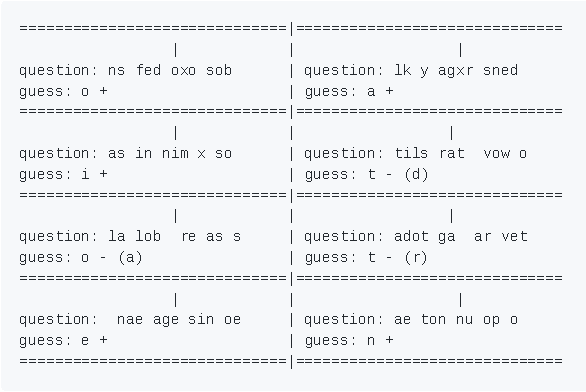
\includegraphics[width=0.6\linewidth]{img/scrabble_denoiser_examples}
  \caption{Input/output examples for the denoiser autencoder in the Scrabble domain.}
  \label{fig:scrabble_denoiser_examples}
\end{figure}

\begin{figure}
  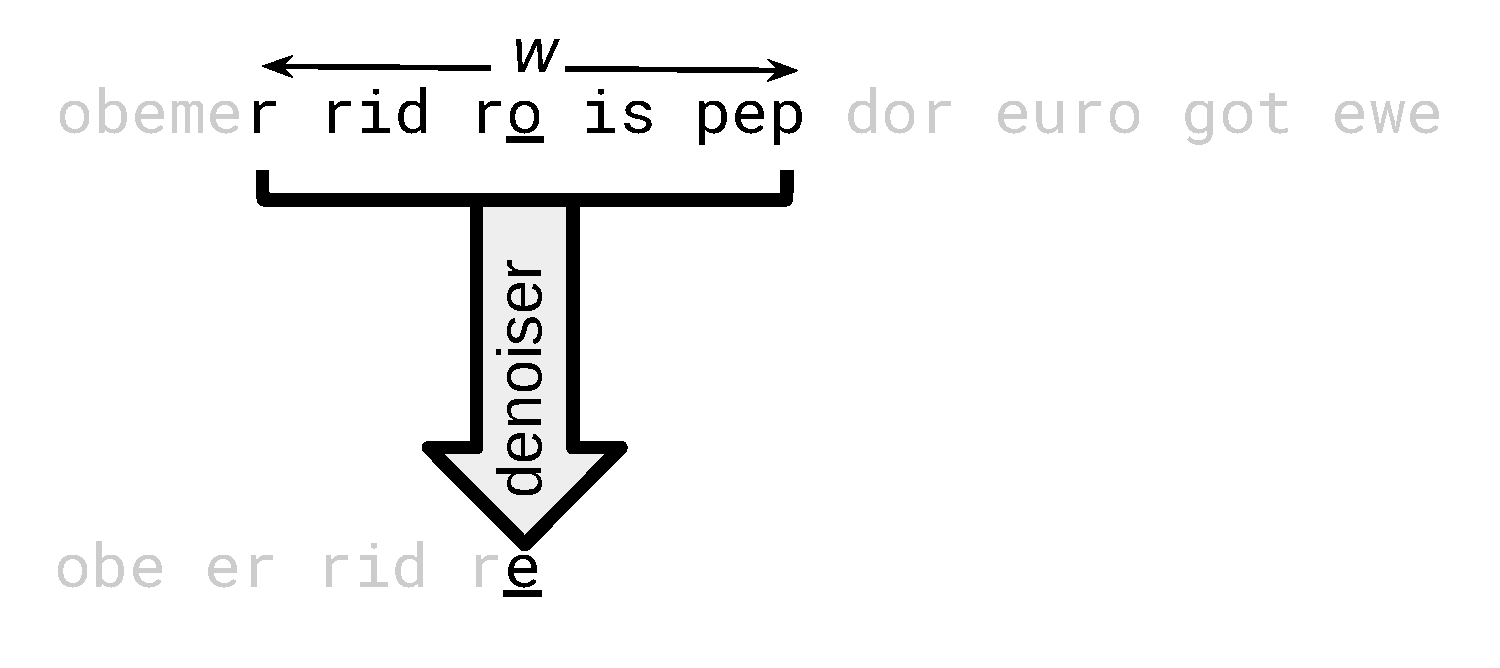
\includegraphics[width=\linewidth]{img/scrabble_denoiser}
  \caption{Illustration of denoising autoencoder in action in the Scrabble domain.}
  \label{fig:scrabble_denoiser}
\end{figure}


For the Scrabble string problem, the denoising autoencoder consisted of: a 9,000-channel 1-dimensional convolution layer with kernel size 3, a ReLU layer, a 100-channel 1-dimensional convolution layer with kernel size 5, a ReLU layer, a 1500-to-1500 fully connected linear layer with bias, a Tanh layer, and a 1500-27 fully connected linear layer with bias.
Initial model weights were drawn from the standard normal distribution.
To generate training data, 20,000 direct-encoded populations of 100-character strings were evolved for 40,000 generations.
During training, input to the autoencoder were 15-character substrings of champion phenotypes with each character encoded as a one-hot vector.
With probability 0.25, the middle character of the presented substring was redrawn.
Over the course of two days, the network was trained for 4 epochs on a GPU-accelerated machine with the Adam optimizer and batch size 256.
Loss was defined as mean square error of the difference between the true identity of the input substring's middle character (before any scrambling) and the predicted identity of that character.
At the conclusion of training, the denoising autoencoder predicted the correct identity of the substring's middle character at a rate of approximately 85\% on testing data.
Example input/output of the denoising autoencoder during training is shown in Figure \ref{fig:scrabble_denoiser_examples}.
For the Scrabble string problem, each site of the 100-character genotype was fed through the denoiser, yielding a new 100-character string that consisted of the denoiser's prediction at each site.
Figure \ref{fig:scrabble_denoiser} illustrates this process.
The denoiser genotype-phenotype mapping was achieved by performing four of these denoising passes on the genotype.

For all Scrabble string experiments, tournament selection with $k = 3$ was used.
No crossover was performed.
(Note, though, that when the bottleneck genotype-phenotype is was employed the genotype is a member of $\mathcal{R}$ so crossover has no effect.)
Mutation was performed by site-wise Gaussian perturbation of the genome.
Mutations scrambled a single, randomly-chosen character in the genotype.
We applied a per-individual mutation rate of 0.2 and a per-site mutation rate of 0.1 while evolving training data for the denoiser.
For all other experiments, we used a per-individual mutation rate of 0.33 and a per-site mutation rate of 0.01.
These particular operator and parameter choices were made mainly by happenstance --- as before, it would be beneficial to repeat these experiments with other operator and parameter choices.

\subsection{Evolvability Signature}
Tarapore et al. introduced an evolvability measure that enables simultaneous inspection of both major aspects of evolvability --- viability and novelty of phenotypic outcomes under mutation \cite{tarapore2015evolvability}.
They forgo use of a scalar metric to describe evolvability, instead reporting evolvability using what they term a ``signature.''
Essentially, the signature is a two-dimensional heatmap presenting the changes in phenotypic form and fitness observed in individual offspring from a single parent.
For a highly evolvable individual, we would expect to see offspring occurring with significant frequency in the corner of the heatmap indicating significant change in phenotypic form with slight or no loss of fitness.
The evolvability signature provides a nuanced snapshot of evolvability, allowing for interaction between the two primary components of evolvability to be visualized.
Such information can be highly diagnostic, for example alerting researchers to phenomena that might appear falsely promising using other metrics, such as genetic changes that alter phenotypic form significantly but at great cost to fitness or genetic changes that are beneficial to fitness but fail to uncover novel phenotypic form.
It is important to note that in these diagrams, fitness increases left-to-right and novelty increases top-to-bottom.
Thus, the parental phenotype would be placed in the upper right of the diagram.
Likewise, mutant phenotypes that are both novel and viable are placed in the lower right of the diagram.
